\chapter{Extended Kalman Filters}
\label{Extended Kalman Filters}

The Extended Kalman Filter (EKF) is one of the non-linear versions of the Kalman Filter. For the most part, the EKF algorithm is nearly identical to the KF algorithm. The critical difference is in linearizing the non-linear state and observation function. The EKF uses the Jacobian to linearly approximate the non-linear function around the mean of the Gaussian distribution. Skipping this step would result in the transformed data being non-Gaussian; though taking the Jacobian enables the transformation to remain Gaussian, it is not exact, resulting in some generalization. Linear approximation through a single point also makes the EKF inefficient when dealing with complex, higher order systems. Because of this, the model is highly subject to error, which can be somewhat reduced by setting accurate initial values. Though these flaws exist, the EKF performs strongly with applications of real time spatial fields, including navigation and positioning systems.  \\

 \begin{figure}[h]
    \centering
    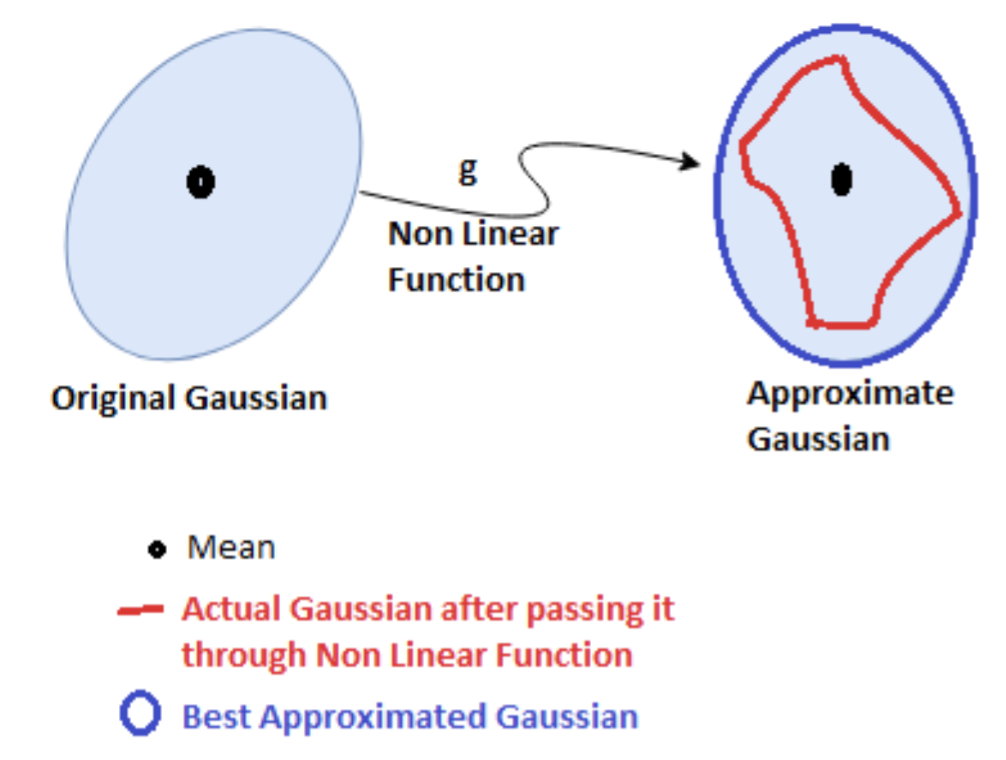
\includegraphics[scale = 0.4]{EKF.png}
    \caption{Overview of how the EKF approximates the Gaussian distribution using the mean after the system has been transformed by a nonlinear function.}
    \end{figure}
    
\clearpage

\section{Extended Kalman Filter Algorithm}
Similar the the KF, the EKF has two main models:
\begin{align*}
&\text{state model: }  x_{k} = f( x_{k-1}) + w_{k-1}\\
&\text{data model: }  \hat y_k = h( x_k) + v_k,
\end{align*}
where $x_k$ is the state vector at time $k$, $f$ is the vector-valued non-linear transformation function, $w_k$ is the process noise at time $k$ such that $w_k = \mathcal{N}(0, Q)$ or  gaussian white noise with covariance $Q$, $h$ is the vector-valued nonlinear observation function, and $v_k$ is the measurement noise at time $k$ such that $v_k = \mathcal{N}(0, R)$ or gaussian white noise with covariance $R$. \\

\noindent The main difference between these models and the models from the KF is that $f$ and $h$ are vector-valued non-linear functions. A prediction can be obtained by taking results from the last time step and transforming them using $f$, which is the non-linear set of ODEs used to describe the system. Similarly, the transformed prediction can be generated by taking the ODEs of states that are measurable, $h$,  to transform the prediction and then add measurement noise. \\ \\
\noindent Although using the non-linear function works for the state and data model, a non-linear function cannot be used in the correction step, such as calculating covariance of the state or the Kalman Gain. To overcome this, the EKF linearizes around the non-linear system by calculating the Jacobian matrix of $f$ and $h$. Recall that the Jacobian matrix allows for the linear approximation of a non-linear system by taking first-order partial derivatives. Let $F$, the Jacobian of $f$, be given by \begin{align*}
      F= \frac{\partial f}{\partial x} =
      \begin{bmatrix}
           \frac{\partial f_1}{\partial x_1} & \hdots & \frac{\partial f_n}{\partial x_n} \\
           \vdots & \ddots & \vdots \\
           \frac{\partial f_n}{\partial x_1}  & \hdots & \frac{\partial f_n}{\partial x_n}
         \end{bmatrix} ,
  \end{align*}
  where $f_i $ is the ODE corresponding to the ith state variable and $x_i$ is the ith state variable. One can see that this results in $F$ being a square matrix. In addition, let $H$ be the Jacobian of $h$, given by
  \begin{align*}
      H = \frac{\partial h}{\partial x} =
     \begin{bmatrix}
           \frac{\partial h_1}{\partial x_1} & \hdots & \frac{\partial h_1}{\partial x_n} \\
           \vdots & \ddots & \vdots \\
           \frac{\partial h_m}{\partial x_1}  & \hdots & \frac{\partial h_{m}}{\partial x_n}
         \end{bmatrix} ,
  \end{align*} 
  where $h_i $ is the ODE corresponding to the ith measurable state variable and $x_i$ is the ith state variable. \\ 
 
    
    
  \noindent Using these linearized versions of $f$ and $h$, the correction step can be applied, making the algorithm similar to the KF. Recall that the algorithm consists of three major components:
\begin{enumerate}
  \item Initialize the state variables
  \item Generate a prediction
  \item Update prediction with measurements from the system.
\end{enumerate}
The recursive component of the filter consists of repeating steps 2 and 3 repeatedly, while step 1 only needs to be done once. For the most part, the EKF is going to be very similar to the KF, with a few exceptions. Details are explained more in depth below. \\

\begin{enumerate}
  \item Begin by initializing the state estimate, $x_0$, and the initial covariance matrix, $P_0$. Similar to the KF, the initial state estimate can be found by 
  \begin{align*}
           \mathbb{E}[x_0]   = \sum^n_{i = a} x_i p_i = [x_a p_a + x_b p_b + \hdots + x_n p_n]^T,
      \end{align*}
      if the system is finite, but otherwise, if it is continuous, it is given by
          \begin{align*}
        \mathbb{E}[x_0]   = \int^n_{a} x_i p_i  dx,
    \end{align*}
 \noindent where  $x_a, x_b, \hdots, x_n$ are the state variable, $p_a, p_b, \hdots, p_n$ is the probability of getting each state variable, and T is the transpose. Initialize the covariance matrix by
    
  \begin{align*}
      P_0 =
      \begin{bmatrix}
           var(x_a)  & \hdots & cov(x_a,x_n) \\
           \vdots & \ddots & \vdots \\
           cov(x_n, x_a)  & \hdots & var(x_n )
         \end{bmatrix} .
  \end{align*}  
  
  Often, $P_0 $ will be initialized as a diagonal matrix with the diagonals being the variance of each state variance and every other value being set to 0.
  
  \item After initializing the model, a prediction can be generated. The prediction step deviates from the Kalman Filter because we can no longer represent the transformation through matrix multiplication because the system is no longer linear. Instead, the prediction is generated by directly applying the last state estimate to the non-linear transformation $f$ and adding process noise $w_k$, which is given by
  \begin{align*}
      x_{k|k-1} = f( x_{k-1|k-1} ) + w_{k-1}.
  \end{align*} 
  
  
  \item The correction step requires transforming the prediction and calculating the Kalman Gain. Begin by linearizing both $f$ and $h$ by calculating the Jacobian. Let $F$ be the Jacobian of $f$ and let $H$ be the Jacobian of $h$, both of which are given by
    \begin{align*}
      F= \frac{\partial f}{\partial x} =
      \begin{bmatrix}
           \frac{\partial f_1}{\partial x_1} & \hdots & \frac{\partial f_n}{\partial x_n} \\
           \vdots & \ddots & \vdots \\
           \frac{\partial f_n}{\partial x_1}  & \hdots & \frac{\partial f_n}{\partial x_n}
         \end{bmatrix}  ,
  \end{align*}
      \begin{align*}
      H = \frac{\partial h}{\partial x} =
     \begin{bmatrix}
           \frac{\partial h_1}{\partial x_1} & \hdots & \frac{\partial h_1}{\partial x_n} \\
           \vdots & \ddots & \vdots \\
           \frac{\partial h_m}{\partial x_1}  & \hdots & \frac{\partial h_{m}}{\partial x_n}
         \end{bmatrix} ,
  \end{align*}
  where $f_i $ is the ODE corresponding to the ith state variable, $h_i$ is the ODE corresponding to the ith measurable state variable, and $x_i$ is the ith state variable. \\
  
  \noindent Using $F$ and $H$, one can now calculate the state covariance and the Kalman Gain.  Recall that the Kalman Gain is a method to determine whether to place more weight on incoming measurements or the system's model. $P_{k | k - 1}$, can be found by
    \begin{align*} 
        P_{k | k -1} = F P_{k-1|k - 1} F^T + Q_{k-1} ,
        \end{align*}
       where $F$ is the Jacobian of the nonlinear state function, $P_{k - 1} $ is the state covariance at the last time step, $T$ is the transpose, and $Q$ is the process noise covariance. Using $P_{k | k - 1}$, calculate the Kalman Gain by
         \begin{align*} 
        K_k = P_{k | k - 1} H^T (H P_{k | k - 1} H^T + R_k)^{-1},
    \end{align*}
    where $H$ is the Jacbian of the nonlinear observation matrix, and $R$ is the measurement noise covariance.
    Recall that $H$ and $F$ are linear approximations of $f$ and $h$. Therefore, it is assumed that there is some amount of error when calculating the Kalman Gain. \\
 
    \noindent  The next component of the correction step is to transform the prediction to compare with incoming measurements from the system, $y_k$. The transformed prediction, $\hat y_k$, is given by
    \begin{align*}
        \hat y_k = h( x_{k|k-1} ) + v_k,
    \end{align*}
   where $h$ is the vector-valued non-linear observation function and $v_k$ is measurement noise. The equation can be updated by 
     \begin{align*} 
        x_{k|k} = x_{k |k-1} + K_k(y_{k} - \hat y_{k}).
    \end{align*}
    
    \noindent Finally, update the covariance matrix, $P_k $, which will be used in the next iteration of the filter. $P_k $ can be updated by
    \begin{align*} 
        P_{k|k} = (I - K_k H) P_{k | k-1},
    \end{align*}
    where $I$ is the identity matrix, $K_k$ is the Kalman Gain at time $k$, $P_{k | k-1}$ is the covariance matrix given the last time step, and $H$ is the Jacobian of the nonlinear observation matrix. \\
\end{enumerate} 
\clearpage
\begin{center}
\begin{table}
\centering
\caption{Description of all variables in the Extended Kalman Filter} \label{tab:sometab}
\begin{tabular}{ |p{2cm}||p{5cm}|p{2cm}| }
    \hline
    \multicolumn{3}{|c|}{Variables in the Extended Kalman Filter } \\ 
    \hline
    Variable & Description & Dimensions \\
    \hline
    $x$ & State variables  & $x \times 1$ \\
    $\hat y$ & Transformed state vector  & $y \times 1$ \\
    $y$ & Actual system measurement(s) & $y \times 1$ \\
    $v$ & Measurement noise & $y \times 1$\\
    $w$ & Process noise & $x \times 1$\\
    $f$ & Non linear state function  & $x \times 1 $  \\ 
    $F$ & Jacobian of $f$  & $x \times x $  \\ 
    $h$ & Non linear observation function & $y \times 1$\\
    $H$ & Jacobian of $h$ & $y \times x$\\
    $K$ & Kalman Gain  & $x \times y$\\
    $Q$ & Process noise covariance  & $x \times x$ \\
    $R$ & Measurement noise covariance &  $y \times y$\\
    $P$ & Covariance matrix & $x \times x $  \\ 
    \hline
\end{tabular}
\end{table}
\end{center}
